\section{\K 电路的基本定律}

\begin{wrapfigure}{r}{6cm}
\centering
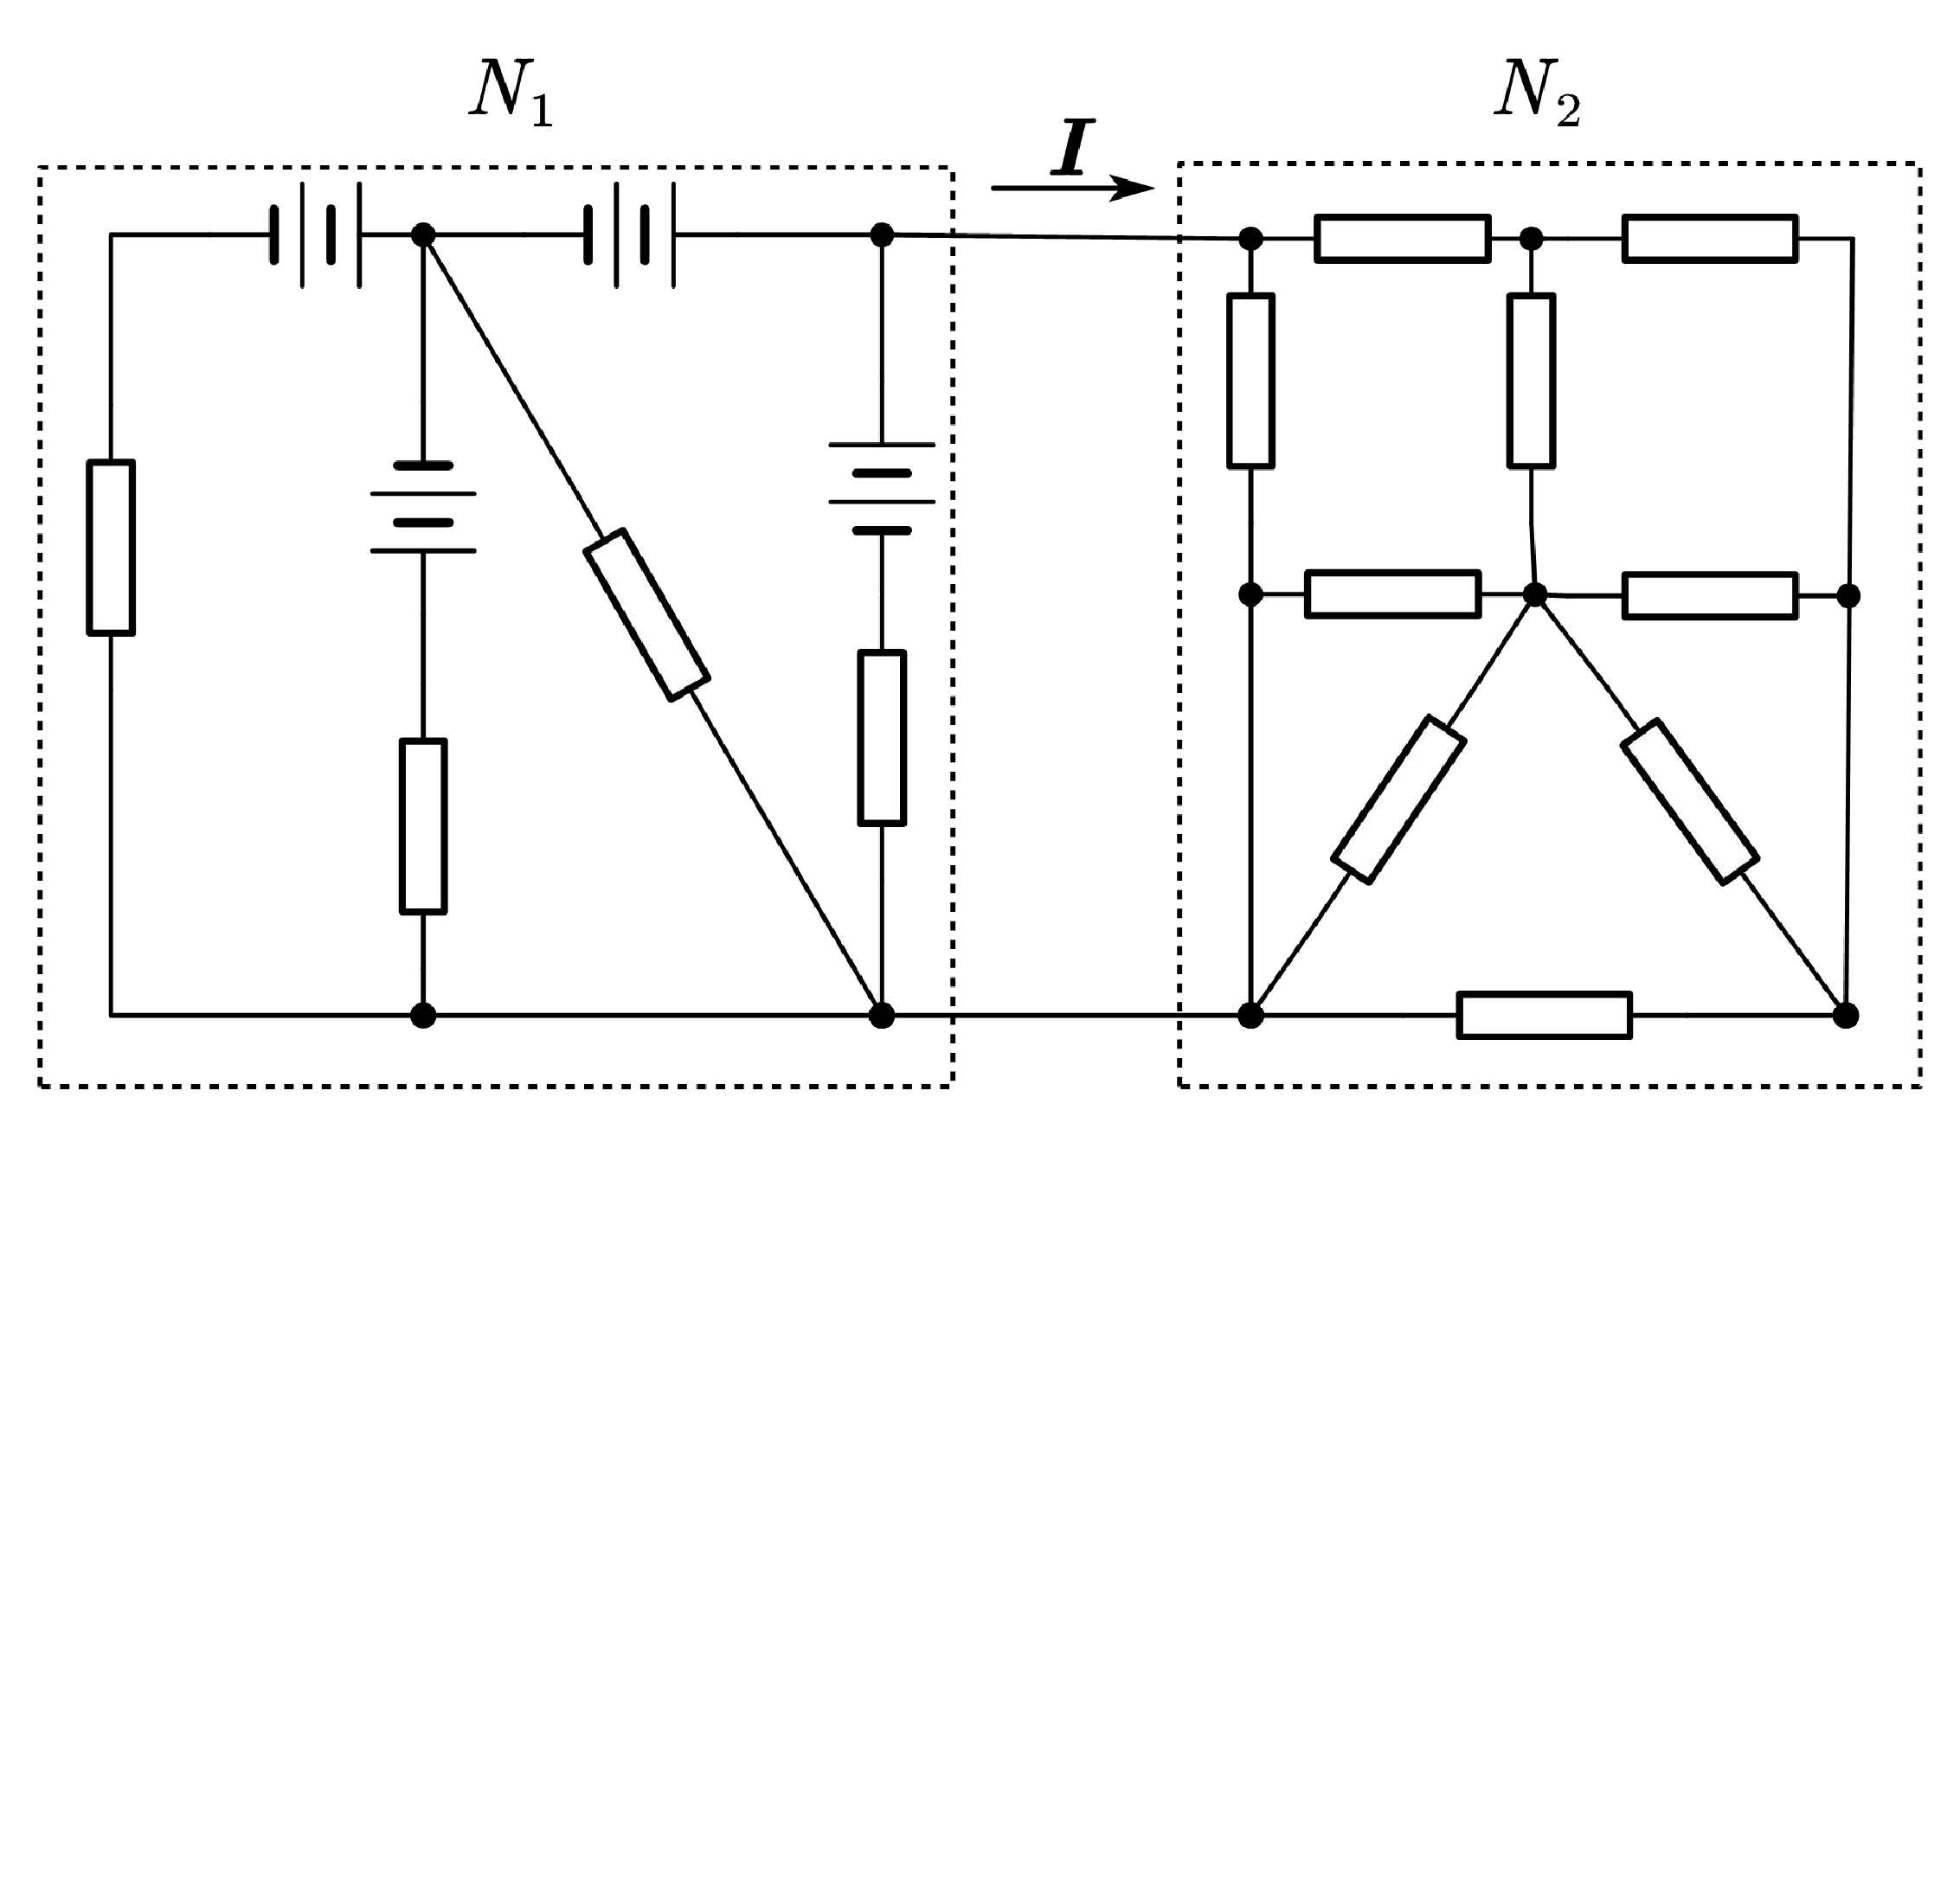
\includegraphics[width=0.36\textwidth]{复杂电路.pdf}
\caption{复杂电路}
\end{wrapfigure}
\textbf{复杂电路}:不能用电阻的串并联等效化简的电路.一般复杂电路有五种求法:
\begin{enumerate}
    \item 支路电流法
    \item 电压源电流源互换
    \item 节点电压法
    \item 叠加原理
    \item 戴维宁定律、诺顿定律
\end{enumerate}
\textbf{支路}:电路中流经同一电流的分支.

\textbf{节点}:三条或三条以上支路的连接点.

\textbf{回路}:由支路组成的闭合路径.

\textbf{独立回路}:至少含有一条其他所有回路都不含有的支路,回路独立与否具有相对性,同时它决定了回路方程的独立性.

\textbf{绕行方向}:回路的绕行方向由人为规定.

\textbf{网孔}:内部不含支路的回路.如图\ref{fig:网孔}所示的,由$l_1$、$l_2$或$l_2$、$l_3$组成的回路即为\textbf{网孔},而由$l_1$、$l_3$组成的回路\textbf{内部}有$l_2$这个支路,因此它不是网孔.\textbf{网孔等价于独立回路},换言之,若回路是网孔,那它必然独立;如果回路独立,那么它必然是网孔.
\begin{figure}[htbp]
    \centering
    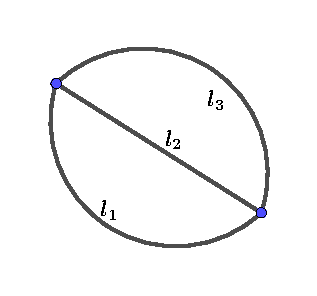
\includegraphics[scale=0.8]{网孔.pdf}
    \caption{网孔}
    \label{fig:网孔}
\end{figure}

\begin{theorem}[基尔霍夫定律]
    \textbf{基尔霍夫第一(电流)定律}:流进直流电路任意节点的电流等于从该节点流出的电流
    \begin{equation}
        \sum_{k=1}^n{I_k}=0
    \end{equation}
    $I_k$为第k个进入(+)或离开(-)此节点的电流

    \textbf{基尔霍夫第二(电压)定律}:沿着闭合回路所有元件两端的电势差(电压)的代数和等于零:
    \begin{equation}
        \sum_{k=1}^m{U_k}=0
    \end{equation}
    m是此闭合回路的元件数目,$U_k$是元件两端的电压,电势升高取正(+),电势降低取负(-).
\end{theorem}
\hl{广义KCL/KVL}:利用二端网络理论我们可以导出广义上的基尔霍夫定律,例如,如图\ref{fig:二端网络(简化后)}所示,对于这样的一个复杂电路我们将它的左右看做两个二端网络,左边视作有源二端网络,右边视作无源二端网络,这样我们就能将其简化使用KCL、KVL方程组.
\begin{figure}[htbp]
    \centering
    \begin{minipage}{0.48\textwidth}
        \centering
        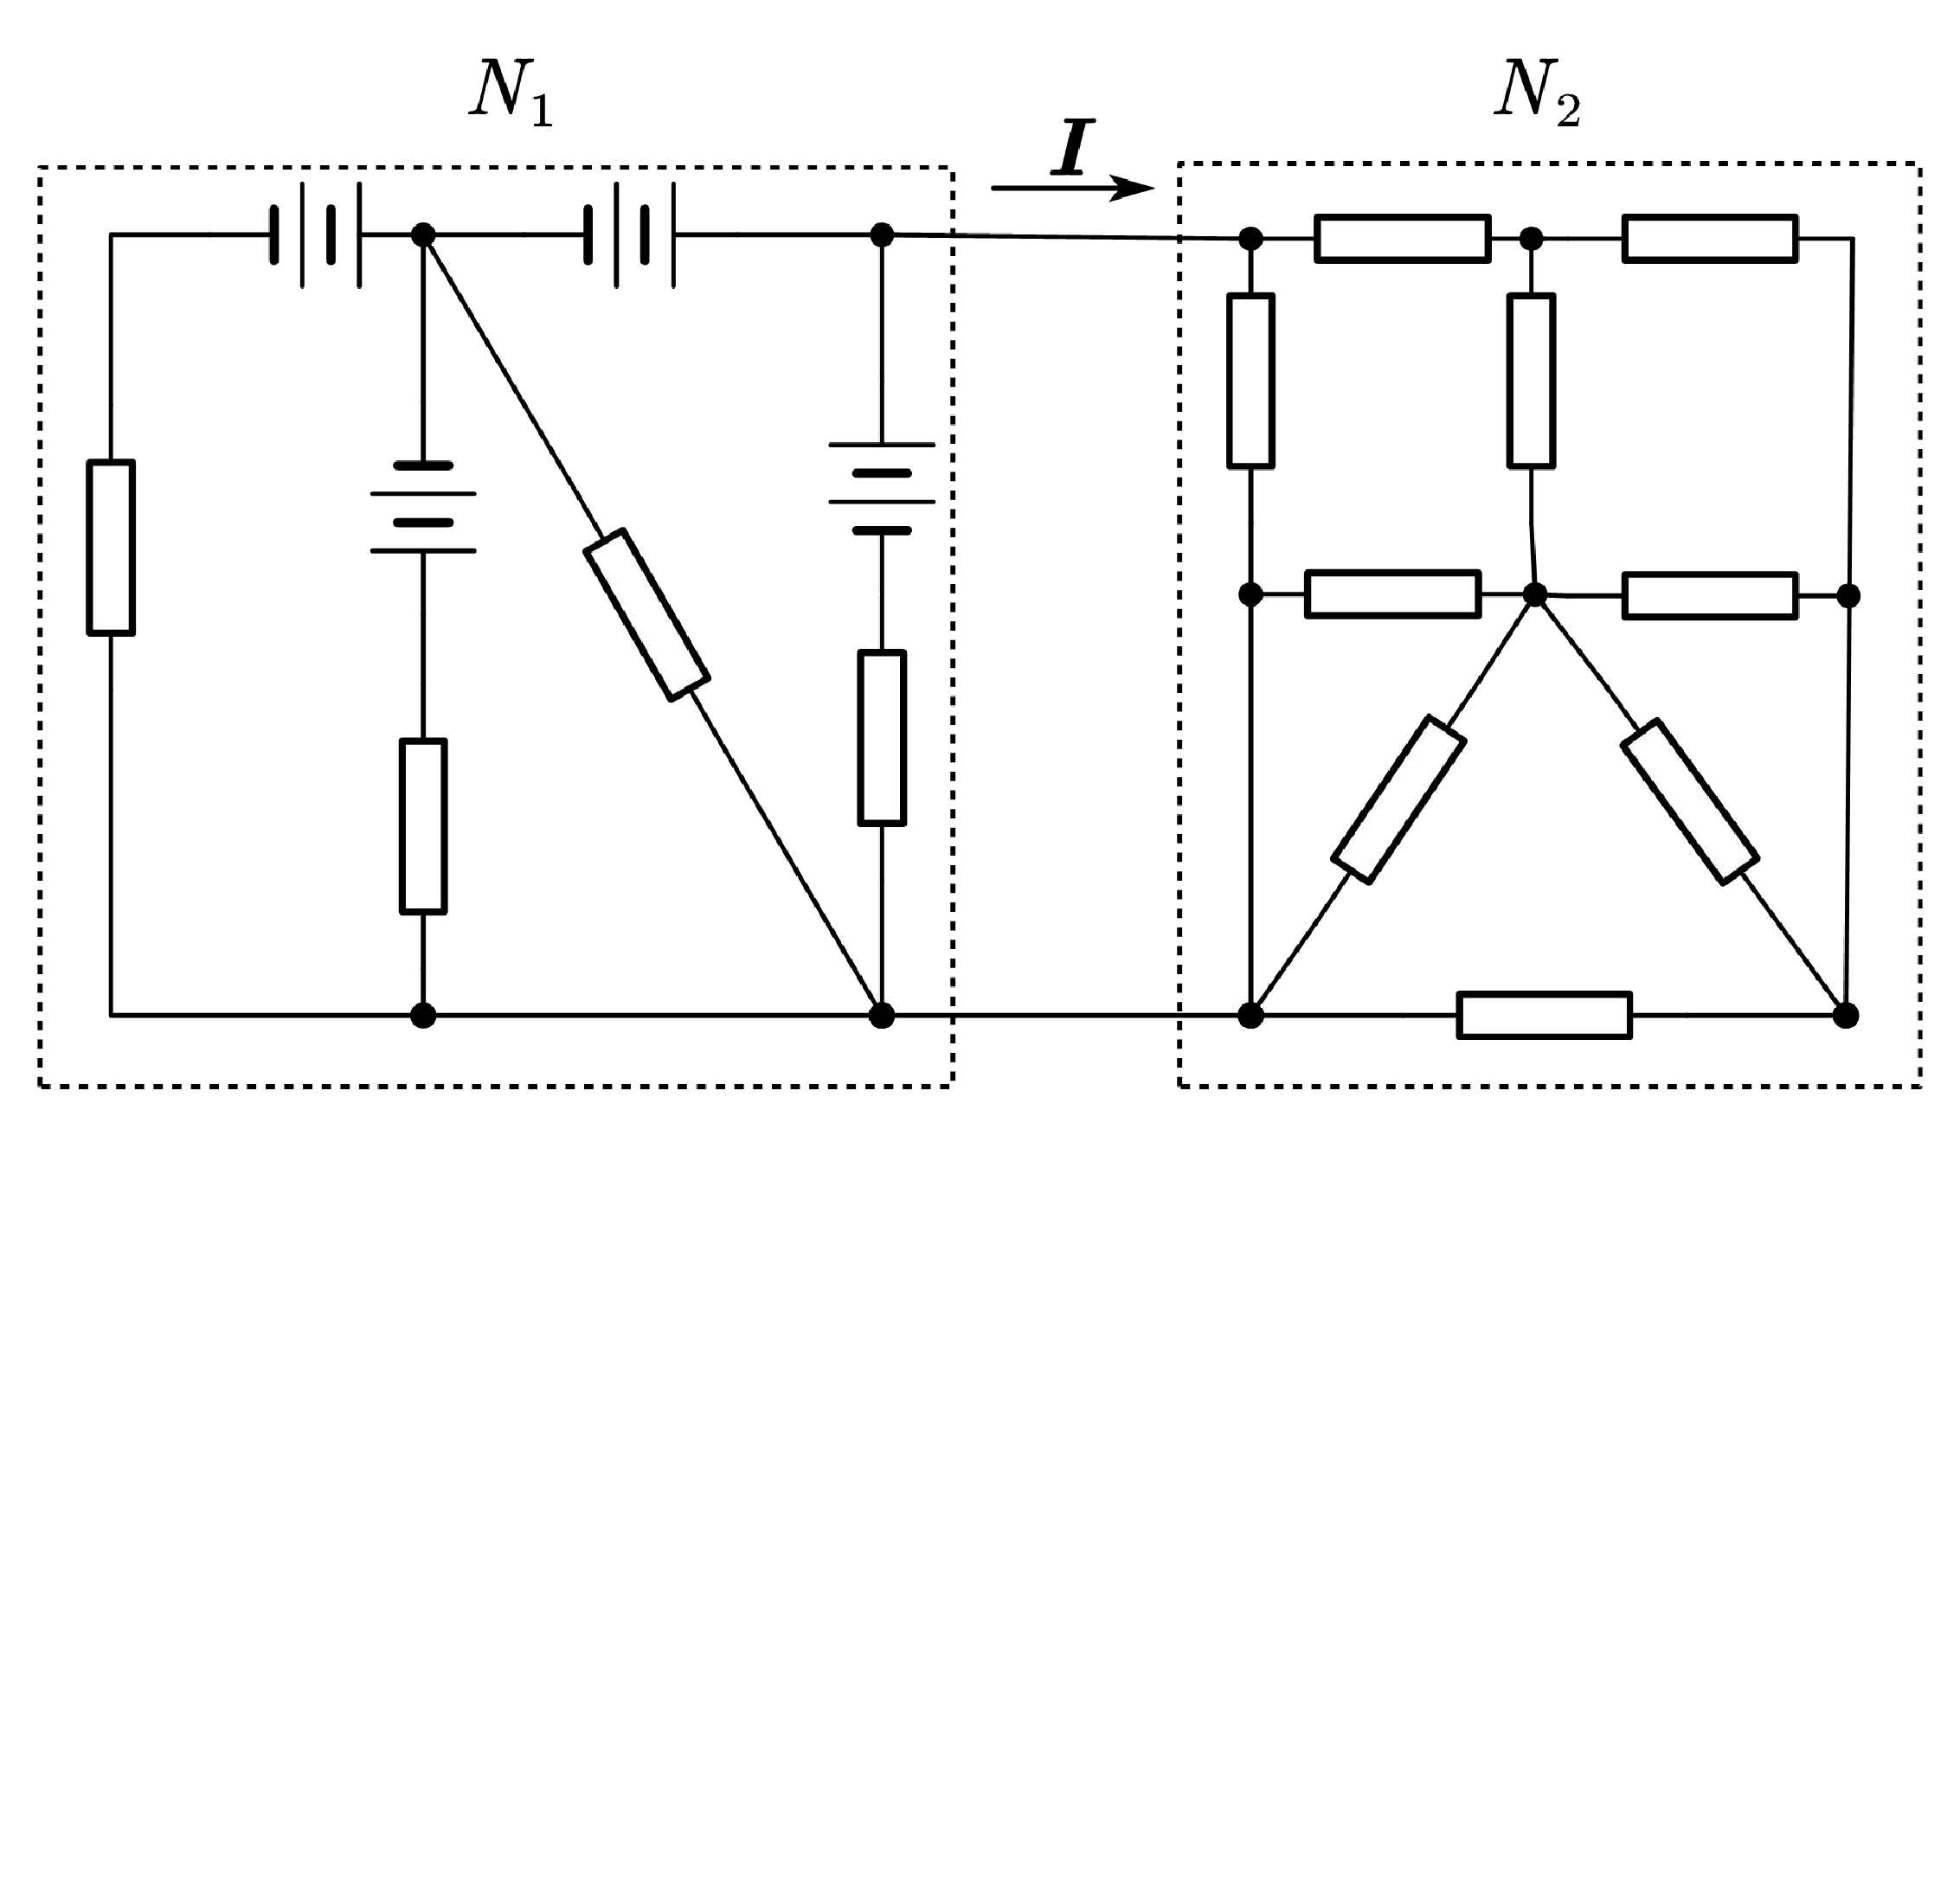
\includegraphics[height=0.16\textheight,width=0.72\textwidth]{二端网络(简化前).pdf}
    \caption{二端网络(简化前)}
    \end{minipage}
    \begin{minipage}{0.48\textwidth}
        \centering
        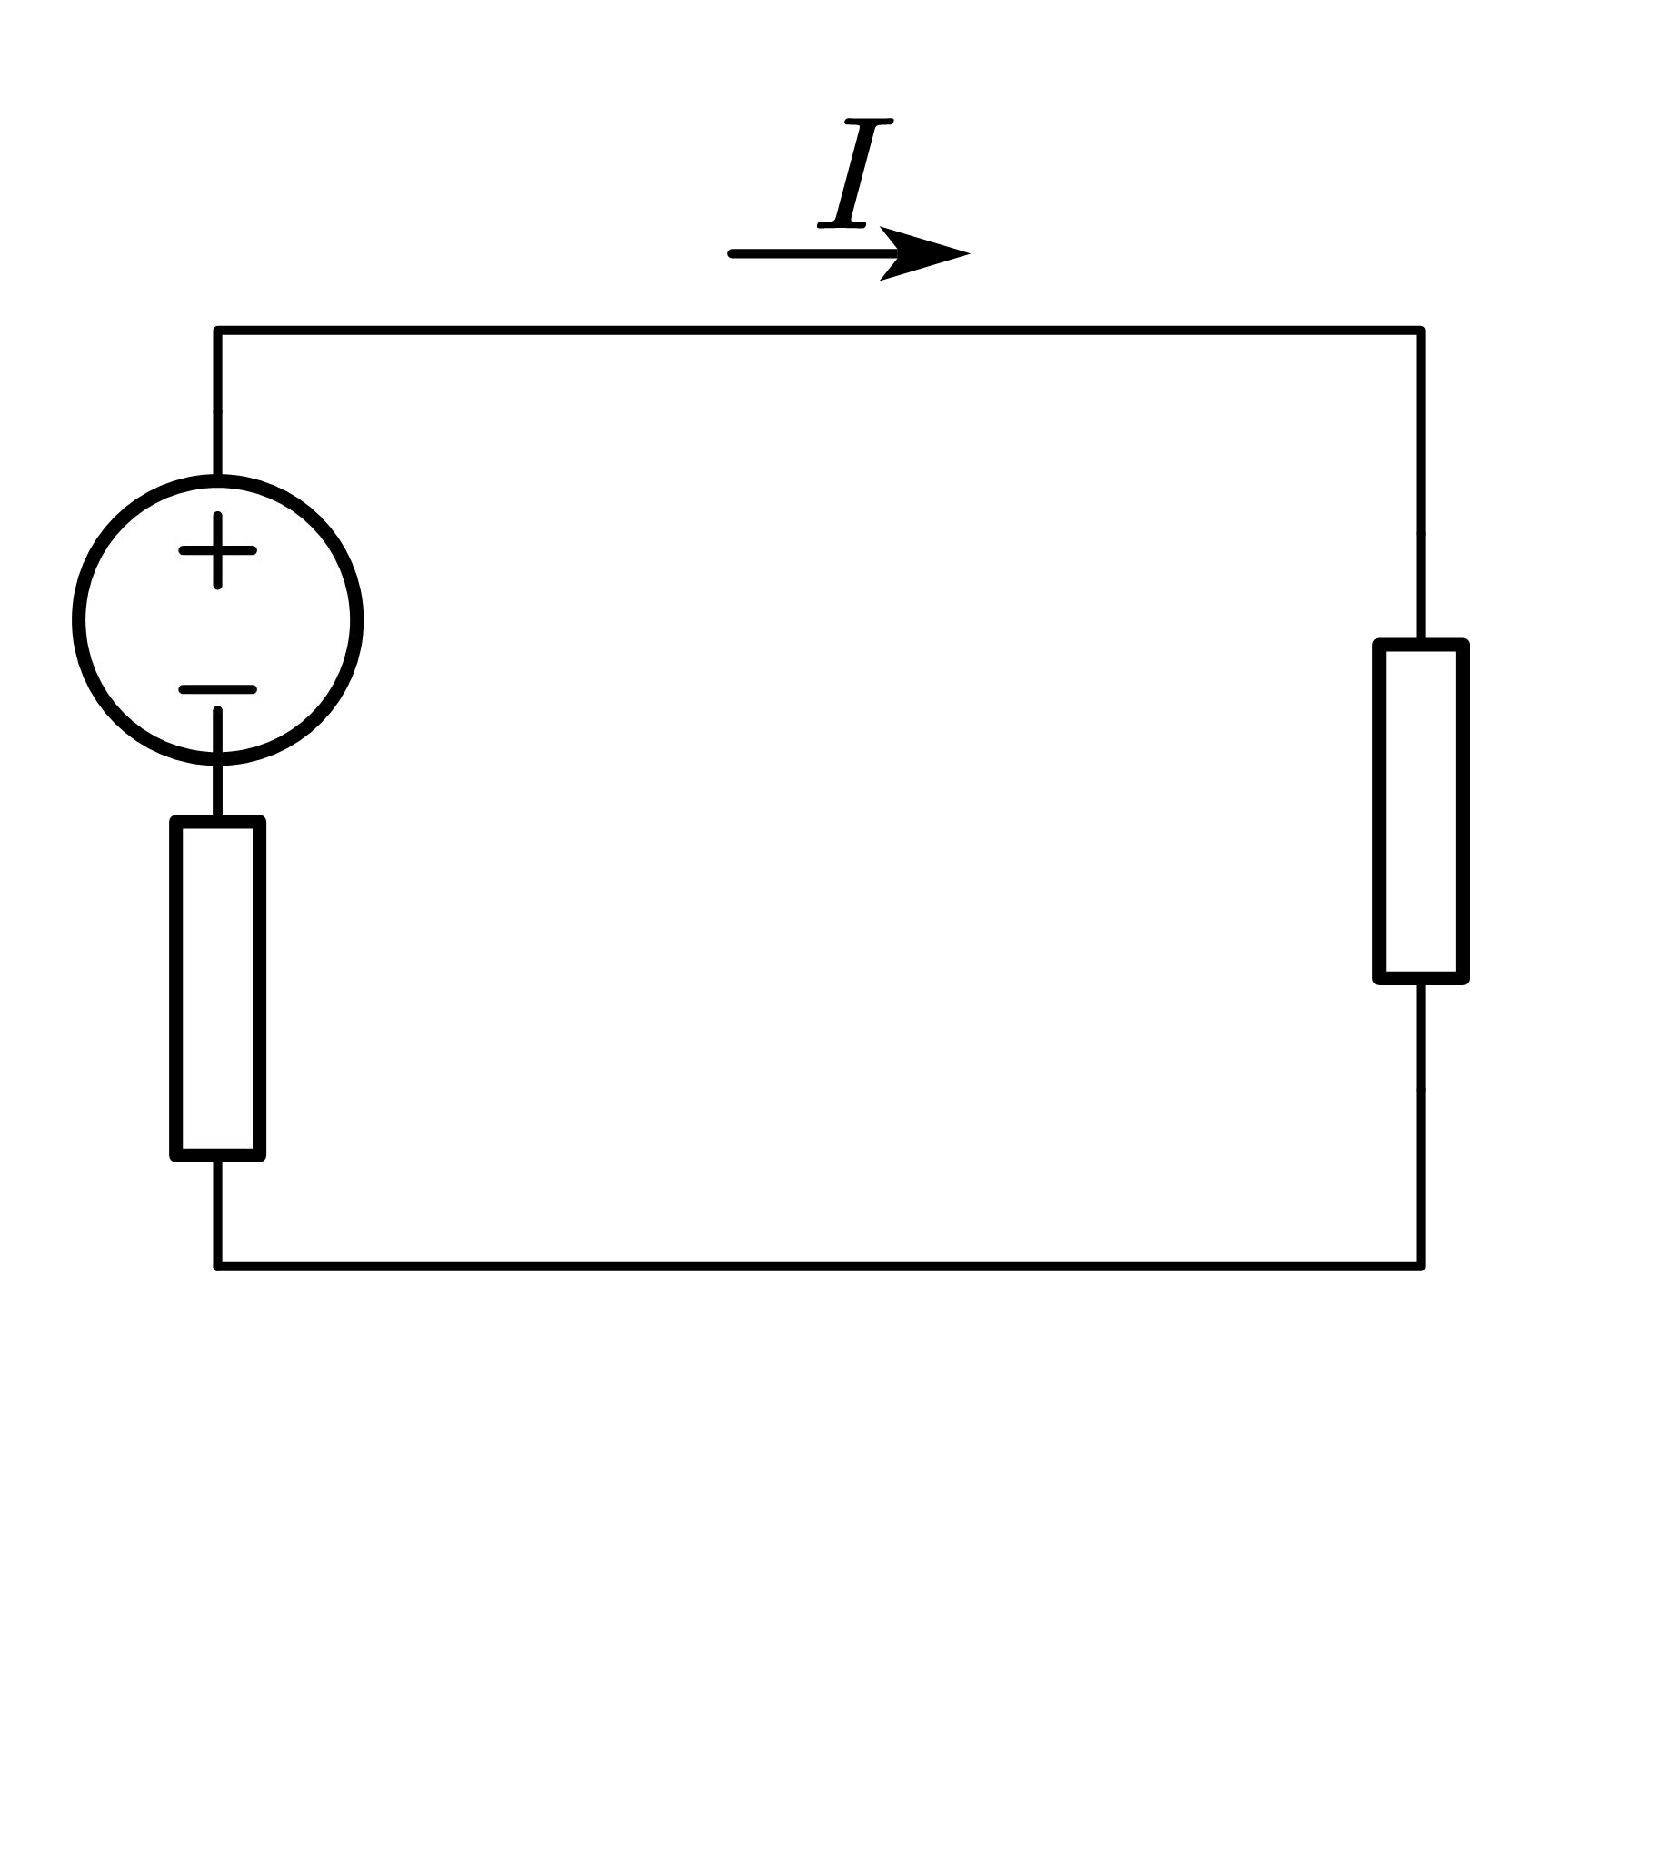
\includegraphics[height=0.16\textheight,width=0.72\textwidth]{二端网络(简化后).pdf}
    \caption{二端网络(简化后)}
    \label{fig:二端网络(简化后)}
    \end{minipage}
\end{figure}


